\chapter{Implementation}
\label{chapter:implementation}

In chapter 3, it was presented an overview of the SmartLighting project, giving an outline of the requirements and use cases. Also, to satisfy the project needs, an overview of the several scenarios of functioning as well as a possible architecture for the system was presented.

The objective for this chapter is to describe the steps and decisions taken, and the reasoning behind the implemented features. It starts in section \ref{implementation:objectives}, by presenting the objectives for the implementation, following by the used technologies on the several components in section \ref{implementation:technologies}. After that, in sections \ref{implementation:devices} and \ref{implementation:rules}, it is presented the standards used to access the devices and to define rules, respectively. Following, in section \ref{implementation:architecture}, the whole system's architecture as well as the functioning of its components is described. 

Since one of the requirements and objectives for this project was the existence of failure handling mechanisms, in section \ref{implementation:scenarios}, it is described the implementation taking into account the several scenarios addressed in the previous chapter. 

\newpage

\section{Objectives}
\label{implementation:objectives}

Although the implementation of the whole solution, presented in chapter \ref{chapter:architecture}, would be optimal to validate the project, it would be unrealistic due to the amount of time necessary to do so and the limited time available for this dissertation. Since some of the features were already implemented, such as a working platform to create and manage rules, a \ac{cep} engine and a simple gateway to communicate with devices through BLE, this dissertation's main focus was in the implementation of gateways capable of implement automation rules, alike to the ones implemented by the CEP engine, as well as give them means to adapt to failing and emergency states. For that reason, was also implemented a gateway manager to act as a monitor for the gateways, being able to control not only the functioning of each one of them as well as manage the distribution of rules and devices throughout the gateways.

Looking at the architecture presented in chapter 3, the component for the user management dashboard was not implemented for the scope of this work. Apart from this, all the features mentioned were implemented and are detailed in the continuation of this chapter.



\section{Adopted  Technologies}
\label{implementation:technologies}

This section aims to discuss the technologies chosen for the different components of the architecture. This choices will be explained taking into account the requirements for this project, however, it is important to note that there are no perfect solutions and, in some cases, several approaches could have been taken.

Since there was a dissertation that already implemented some features like the \ac{cep} engine and the \ac{bm}, some of the technologies used in this dissertation were influenced by past decisions. As far as the \ac{cep} engine concerns, the choice was the WSO2 \ac{cep} \cite{wso2}, since its features addressed all requirements, that such system would need, to fit this project's requirements. For the purpose of this dissertation both the \ac{cep} engine and the \ac{bm} as well as the communication between them, did not affect any of the new implemented features, however, since MQTT was primarily used as the elect protocol for communications in the referred dissertation, the implemented features presented in this work followed the same path.

Finally, it is important to state that the standard used, in SmartLighting project, for both object definition to read and write information to/from devices, and the rules structure, were also maintained and will be described in the following sections. 

\section{Access to Devices}
\label{implementation:devices}

Devices like sensors, which measure environment changes, and actuators, that trigger mechanisms to make changes in that same environment, are fundamental pieces to implement a smart and automated environment. Since there are a huge variety of devices with different characteristics, in order to enable extensibility for the system, the access to those devices, as well as the messages format, should be standardised. In another dissertation for this project, a standard following the IP Smart Objects Alliance guidelines was made and is illustrated in Figure \ref{fig:obj}

\begin{figure}[H]
	\centering
	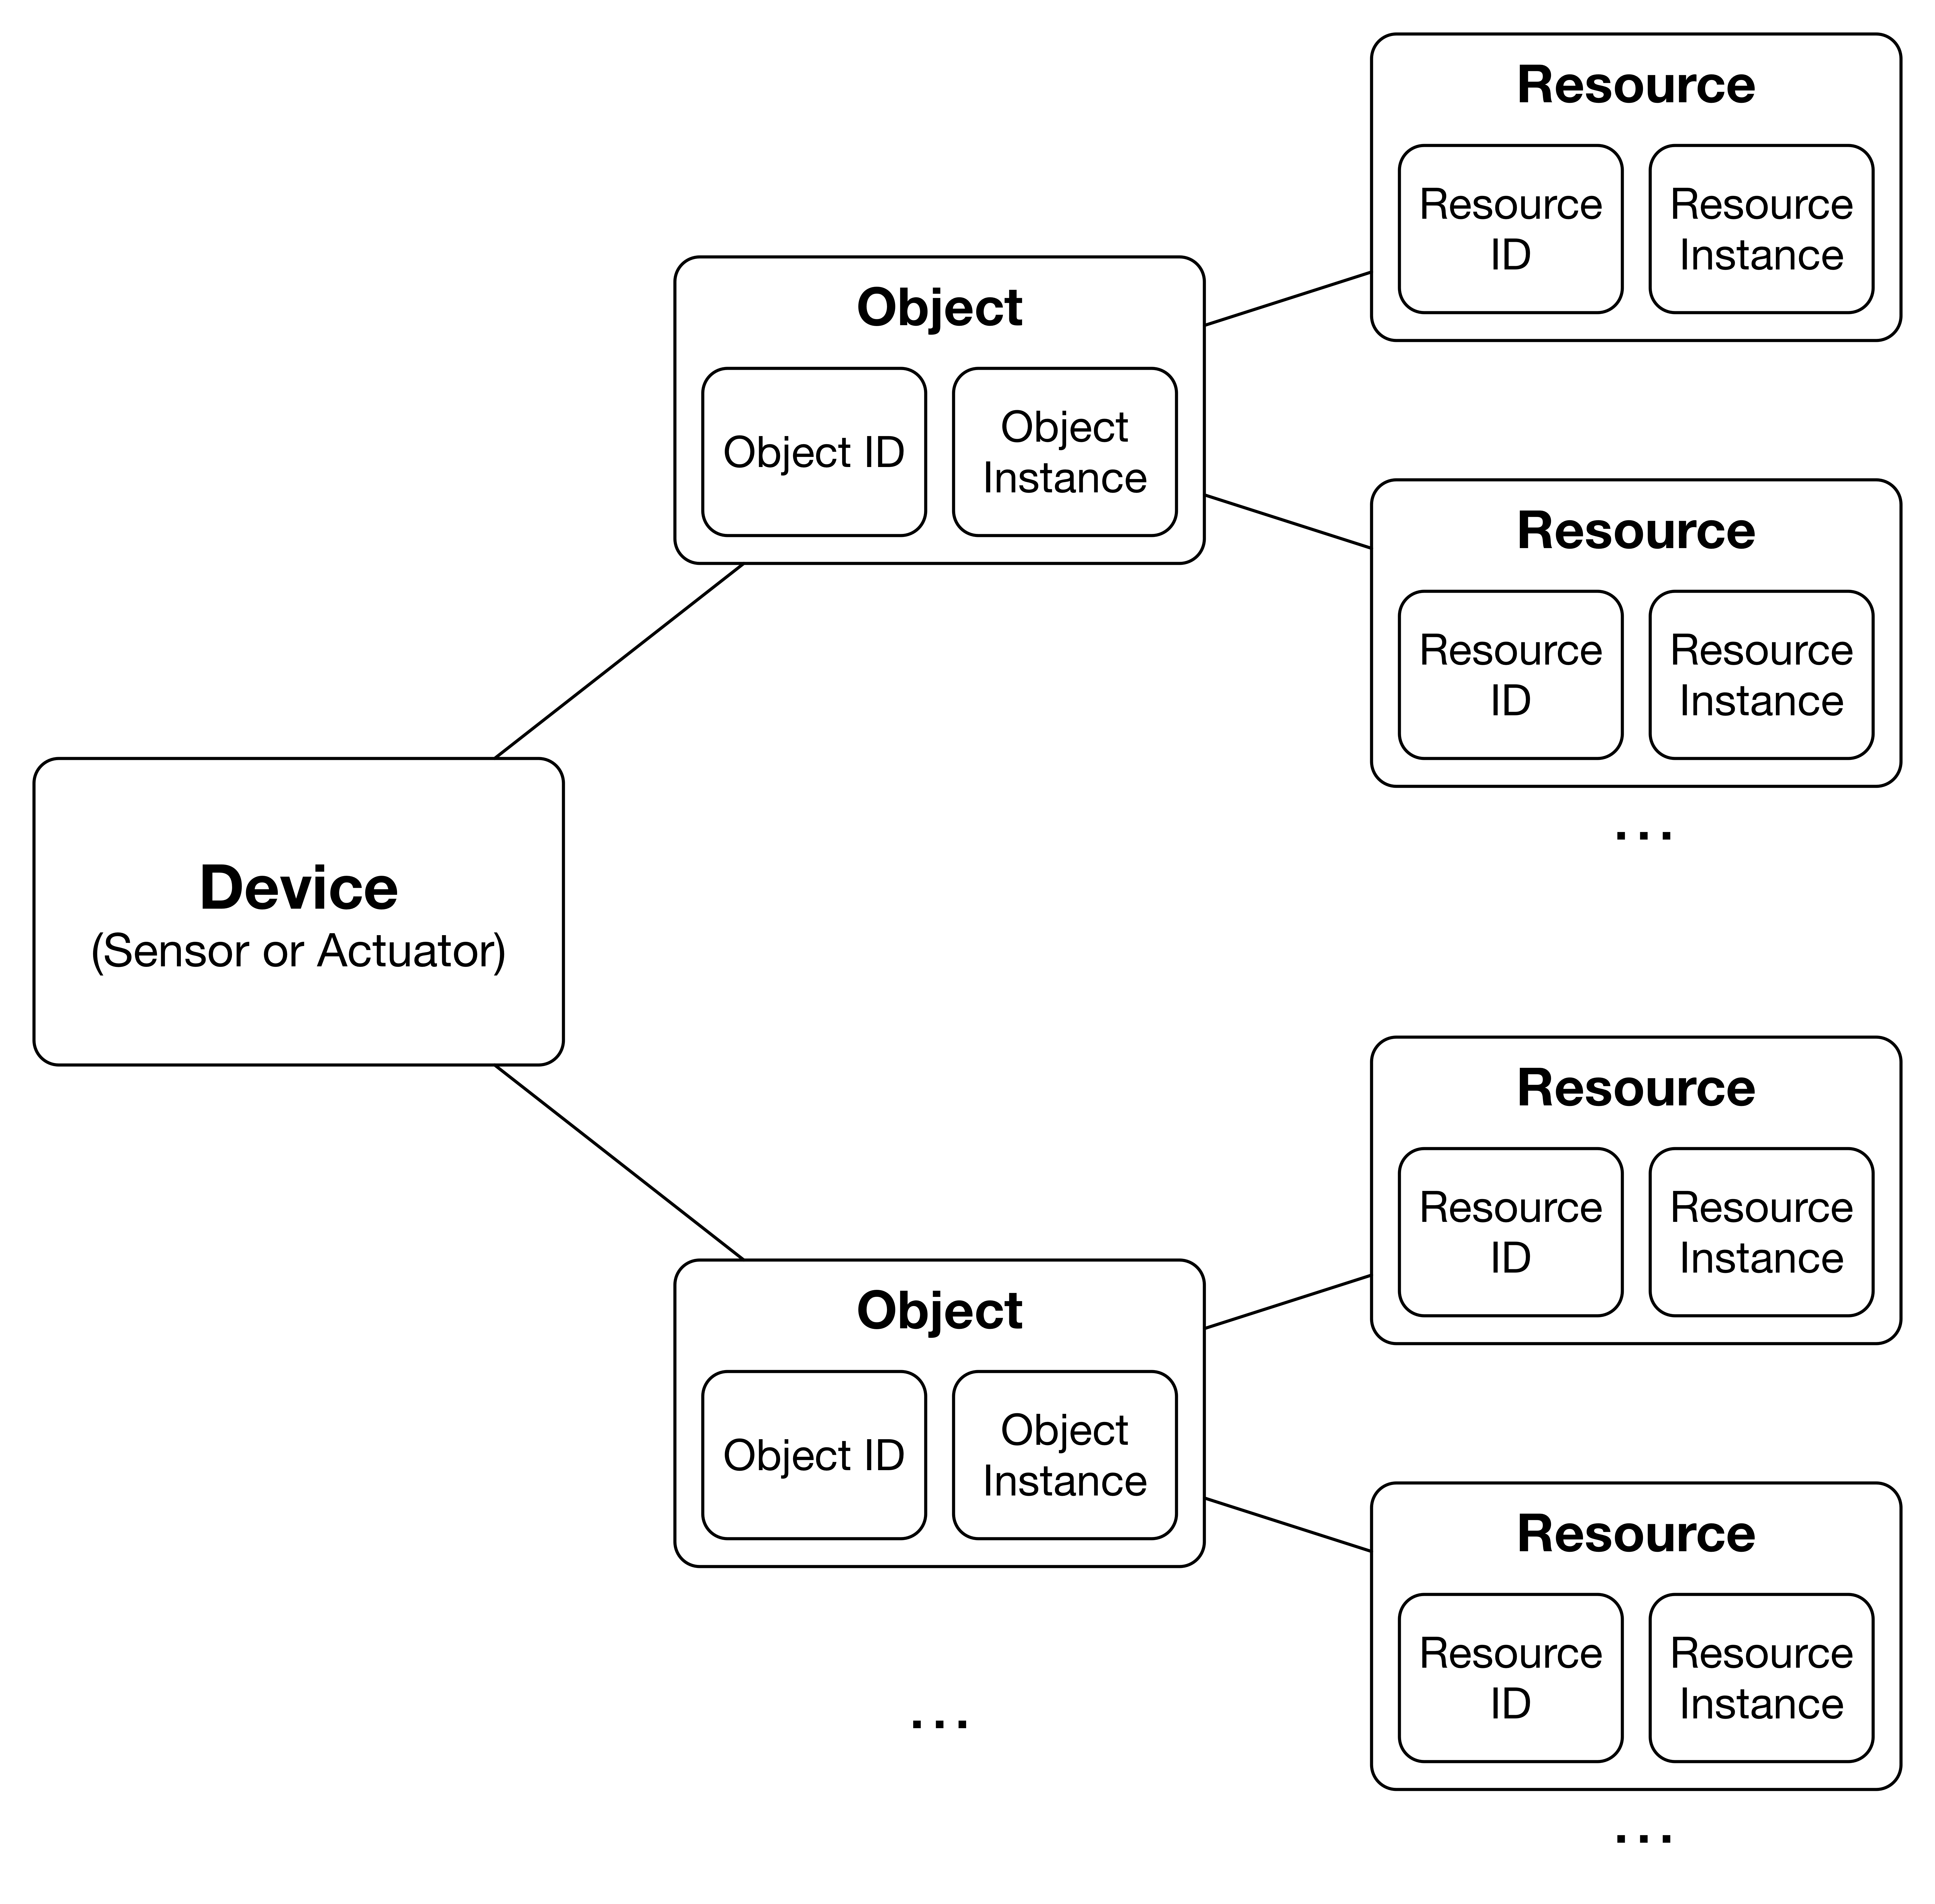
\includegraphics[width=0.9\textwidth]{figures/obj.png}
	\caption{Device objects representation}
	\label{fig:obj}
\end{figure}

Objects are abstract representations of an actuator or sensor type, containing a generic description and some additional information, and each unique object is identified by the object ID. A device can have multiple objects, which represent the different sensing and actuating capabilities it provides. For instance, a device can have objects representing a luminaire actuator, a temperature sensor and a motion sensor.

Inside each object, the information is organized in resources. These represent either values that can be read and/or write, e.g. a sensor configuration parameter or an actuator’s current state, or actions that can be triggered remotely, such as the request to dim a luminaire’s output brightness. Each resource of a given type is also identified by an ID number. Additionally, since a device can contain multiple objects of the same type, as well as objects can contain multiple resources of the same type, e.g. for creating arrays of values, both objects and resources contain an instantiation number for being easily accessed. Figure 4.1 helps understand this representation.

 
\section{Rules Definition}
\label{implementation:rules}
TODO
\section{Architecture}
\label{implementation:architecture}
TODO
\section{Fail Scenarios}
\label{implementation:scenarios}
TODO


